\section{Schematics}

This section contains the system schematics. Figure~\ref{fig:systemSchematics} shows an updated version of the complete system schematic.  The circuit was divided in two two-layered PCBs which will be joined together by spacers and connectors. Figures~\ref{fig:firstBoard} and~\ref{fig:secondBoard} show the two levels of the designed PCB. The PCB has analog components consideration. The accelerometer is placed separately from the other digital components, its power comes directly from the source and it has its own analog ground. SMD Antennas are also considered and are isolated from the ground plane to prevent interference. Power traces are of greater width, supporting up 500mA, while signal lines are of smaller width. 
\subsection{System Schematics}
\begin{figure}[H]
\centering
	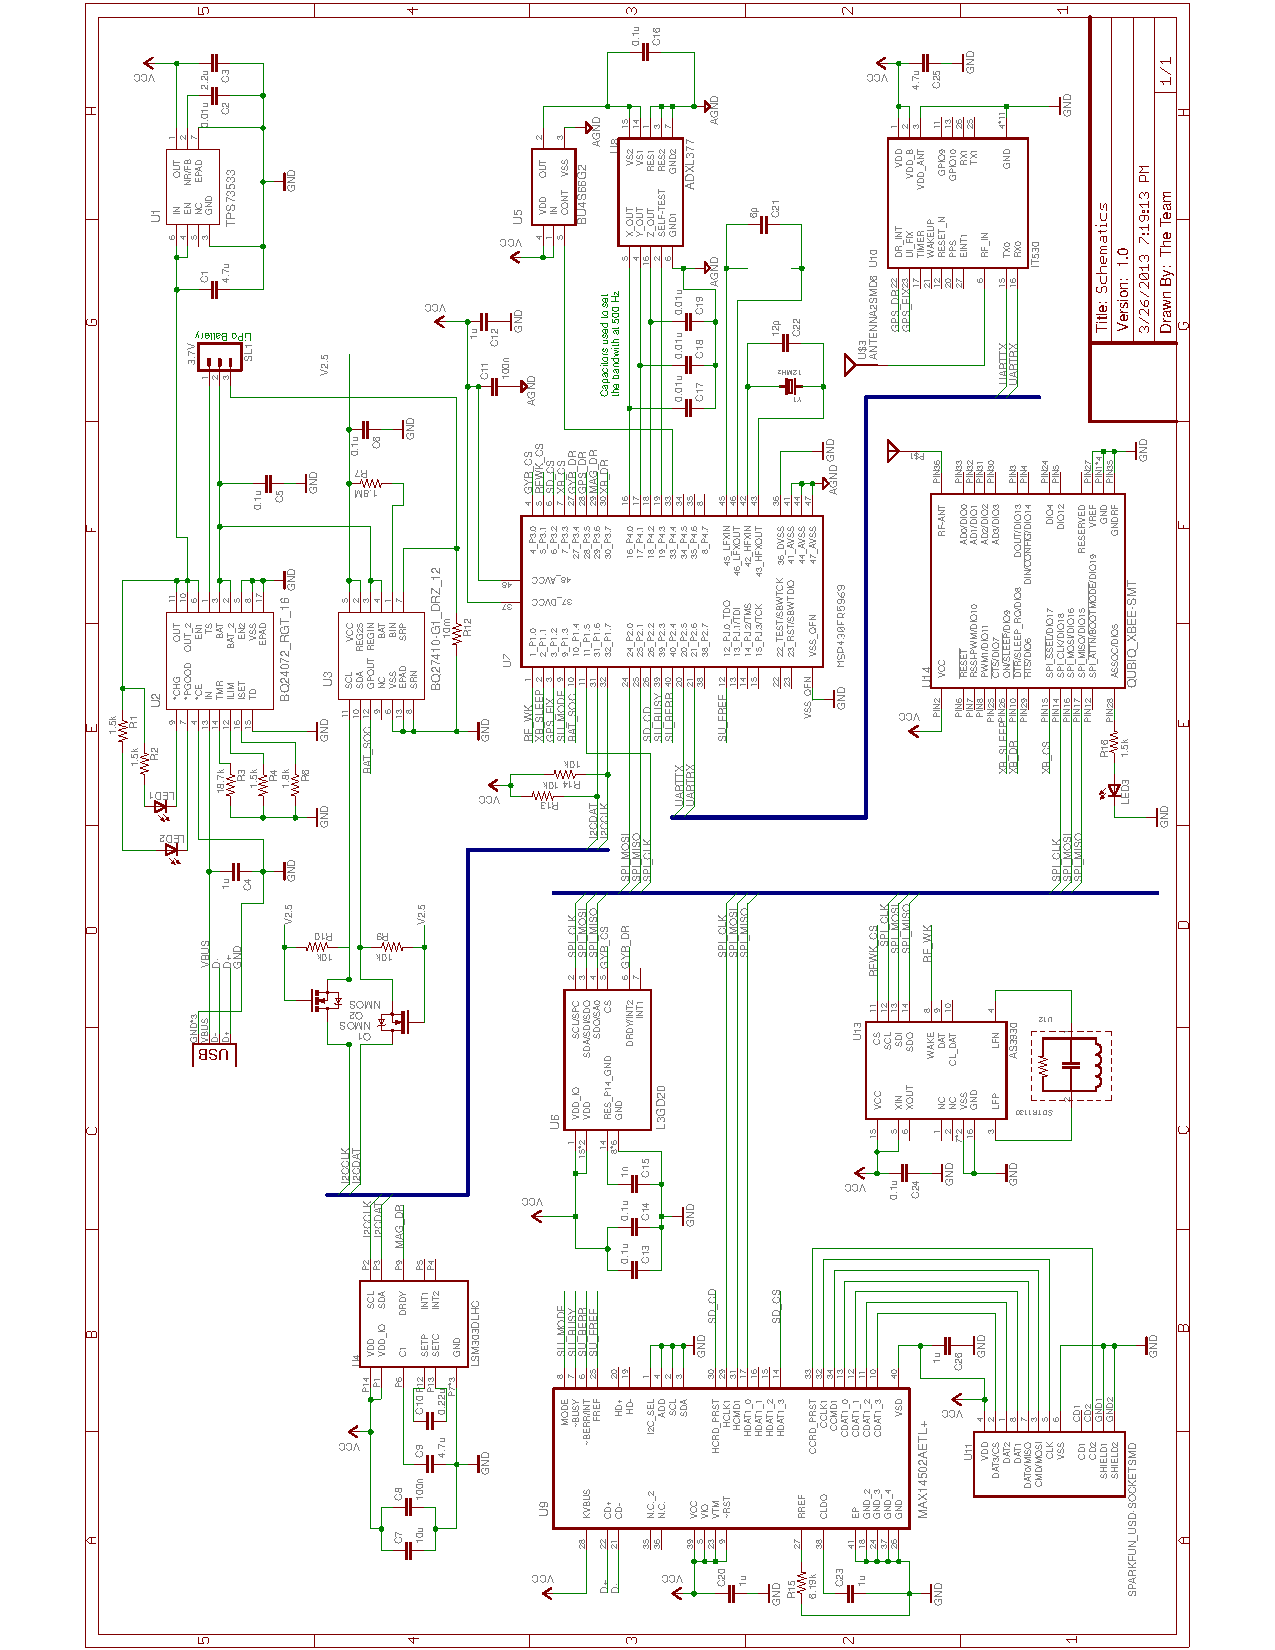
\includegraphics[width=\textwidth]{img/CompleteSchematics}
	\caption{System Schematic \label{fig:systemSchematics}}
\end{figure}

\begin{figure}[H]
\centering
	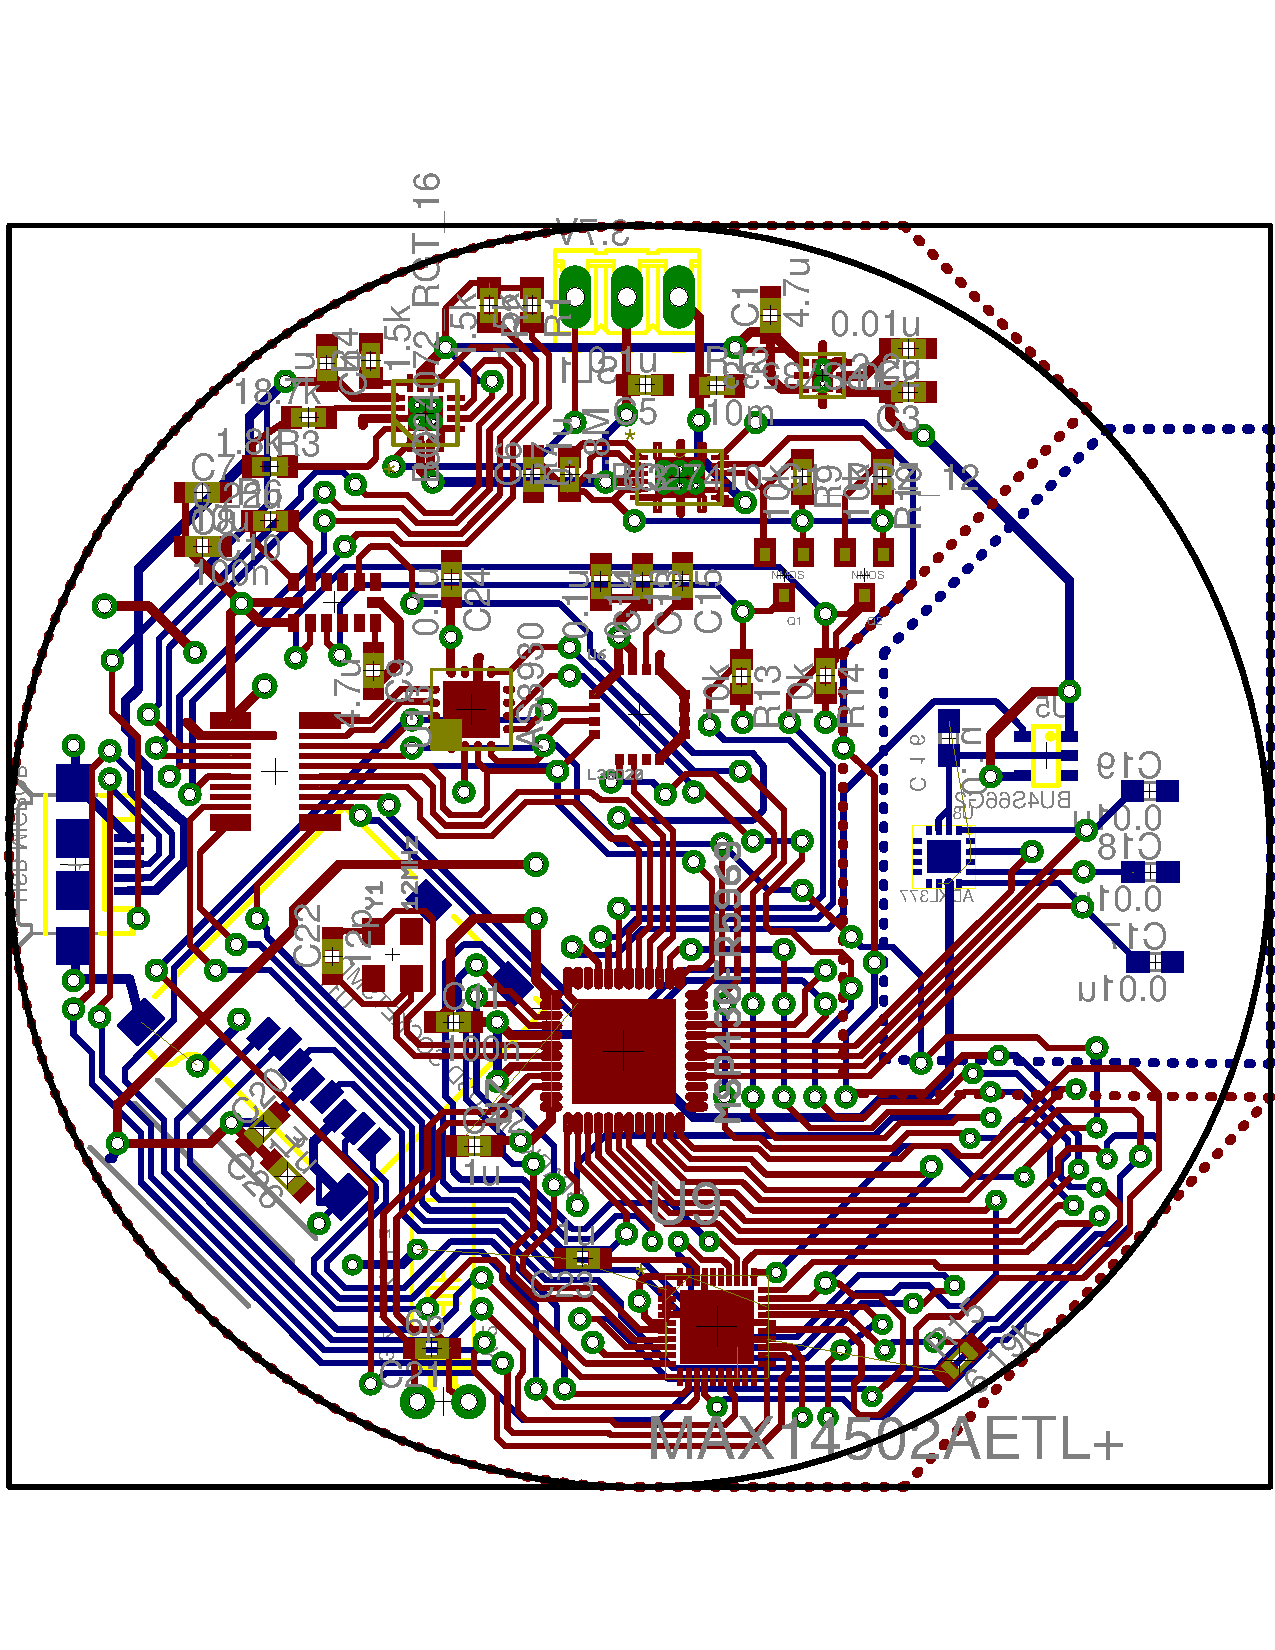
\includegraphics[width=\textwidth]{img/FirstLevelBoard}
	\caption{First Level Board Schematic \label{fig:firstBoard}}
\end{figure}

\begin{figure}[H]
\centering
	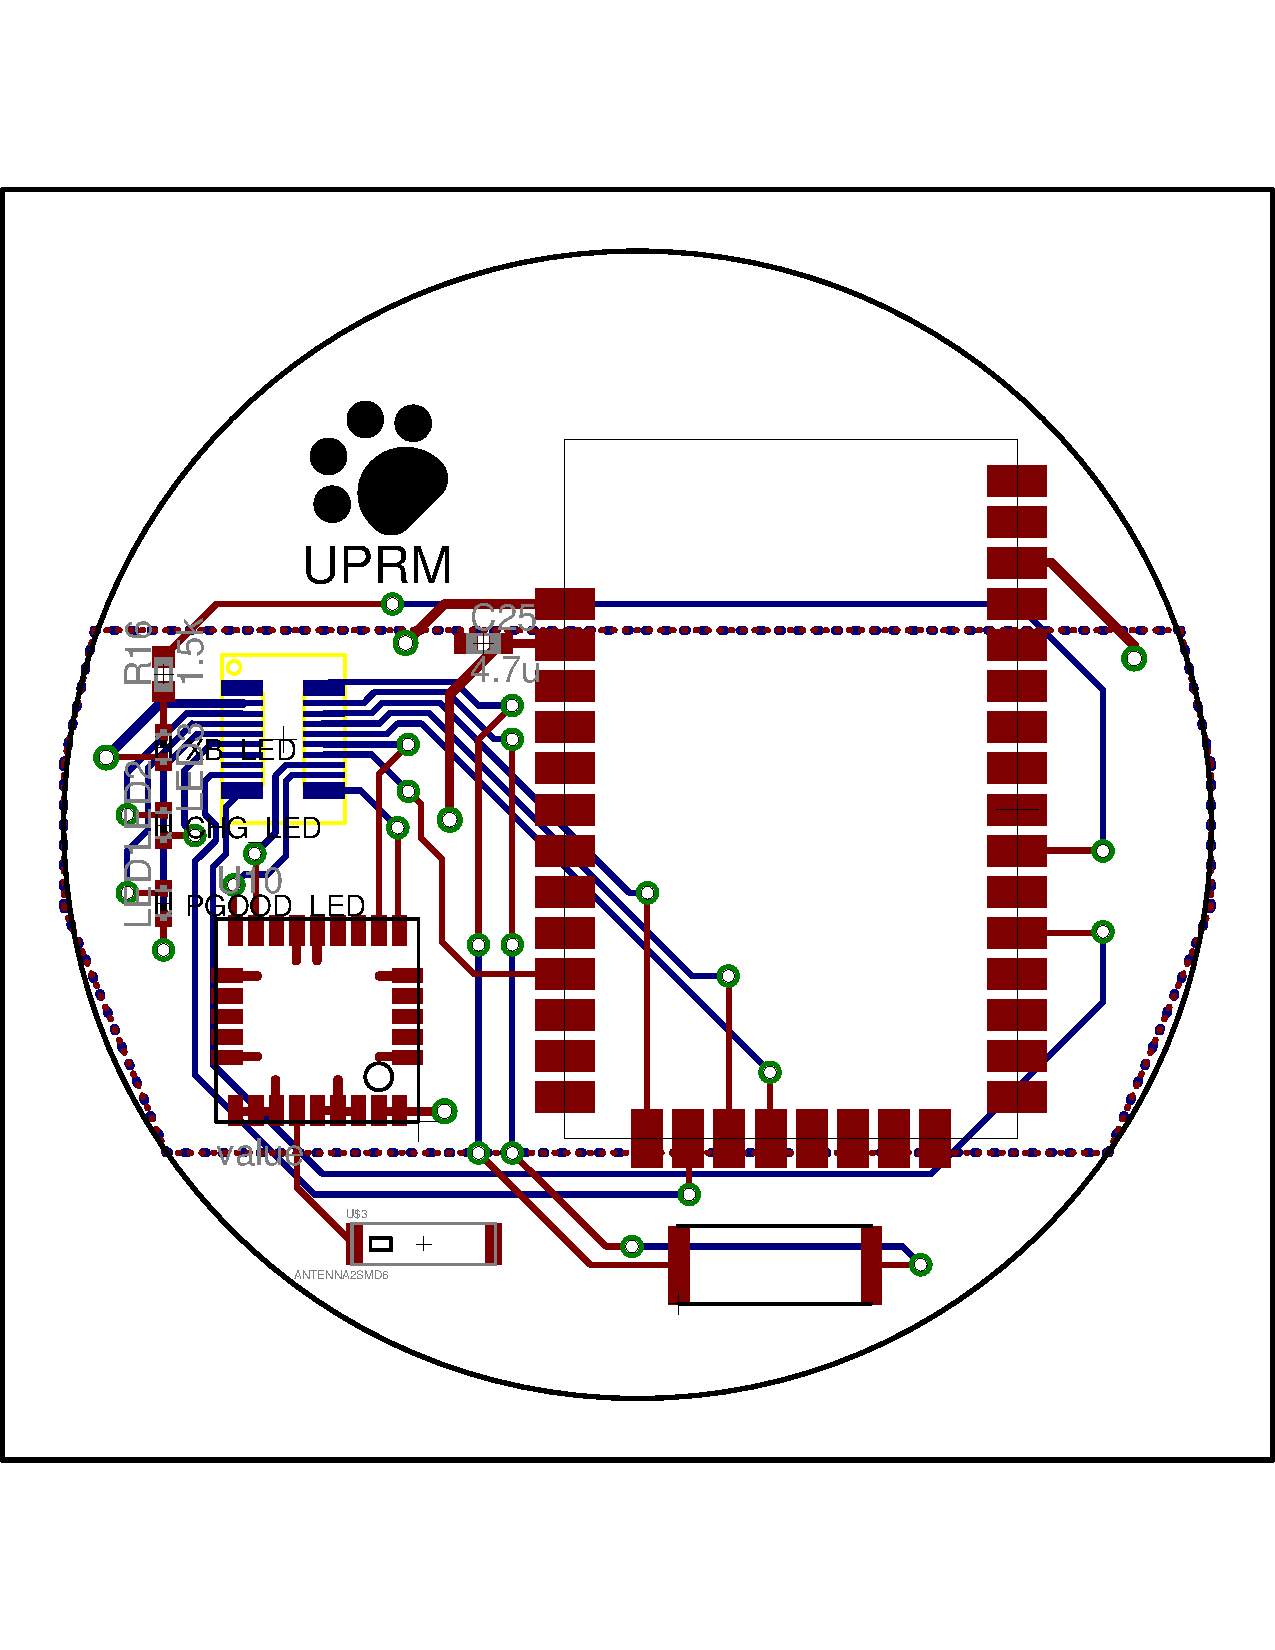
\includegraphics[width=\textwidth]{img/SecondLevelBoard}
	\caption{Second Level Board Schematic \label{fig:secondBoard}}
\end{figure}